\documentclass[]{article}
\usepackage{lmodern}
\usepackage{amssymb,amsmath}
\usepackage{ifxetex,ifluatex}
\usepackage{fixltx2e} % provides \textsubscript
\ifnum 0\ifxetex 1\fi\ifluatex 1\fi=0 % if pdftex
  \usepackage[T1]{fontenc}
  \usepackage[utf8]{inputenc}
\else % if luatex or xelatex
  \ifxetex
    \usepackage{mathspec}
    \usepackage{xltxtra,xunicode}
  \else
    \usepackage{fontspec}
  \fi
  \defaultfontfeatures{Mapping=tex-text,Scale=MatchLowercase}
  \newcommand{\euro}{€}
\fi
% use upquote if available, for straight quotes in verbatim environments
\IfFileExists{upquote.sty}{\usepackage{upquote}}{}
% use microtype if available
\IfFileExists{microtype.sty}{%
\usepackage{microtype}
\UseMicrotypeSet[protrusion]{basicmath} % disable protrusion for tt fonts
}{}
\usepackage[margin=1in]{geometry}
\usepackage{color}
\usepackage{fancyvrb}
\newcommand{\VerbBar}{|}
\newcommand{\VERB}{\Verb[commandchars=\\\{\}]}
\DefineVerbatimEnvironment{Highlighting}{Verbatim}{commandchars=\\\{\}}
% Add ',fontsize=\small' for more characters per line
\newenvironment{Shaded}{}{}
\newcommand{\KeywordTok}[1]{\textcolor[rgb]{0.00,0.44,0.13}{\textbf{{#1}}}}
\newcommand{\DataTypeTok}[1]{\textcolor[rgb]{0.56,0.13,0.00}{{#1}}}
\newcommand{\DecValTok}[1]{\textcolor[rgb]{0.25,0.63,0.44}{{#1}}}
\newcommand{\BaseNTok}[1]{\textcolor[rgb]{0.25,0.63,0.44}{{#1}}}
\newcommand{\FloatTok}[1]{\textcolor[rgb]{0.25,0.63,0.44}{{#1}}}
\newcommand{\CharTok}[1]{\textcolor[rgb]{0.25,0.44,0.63}{{#1}}}
\newcommand{\StringTok}[1]{\textcolor[rgb]{0.25,0.44,0.63}{{#1}}}
\newcommand{\CommentTok}[1]{\textcolor[rgb]{0.38,0.63,0.69}{\textit{{#1}}}}
\newcommand{\OtherTok}[1]{\textcolor[rgb]{0.00,0.44,0.13}{{#1}}}
\newcommand{\AlertTok}[1]{\textcolor[rgb]{1.00,0.00,0.00}{\textbf{{#1}}}}
\newcommand{\FunctionTok}[1]{\textcolor[rgb]{0.02,0.16,0.49}{{#1}}}
\newcommand{\RegionMarkerTok}[1]{{#1}}
\newcommand{\ErrorTok}[1]{\textcolor[rgb]{1.00,0.00,0.00}{\textbf{{#1}}}}
\newcommand{\NormalTok}[1]{{#1}}
\ifxetex
  \usepackage[setpagesize=false, % page size defined by xetex
              unicode=false, % unicode breaks when used with xetex
              xetex]{hyperref}
\else
  \usepackage[unicode=true]{hyperref}
\fi
\hypersetup{breaklinks=true,
            bookmarks=true,
            pdfauthor={},
            pdftitle={Rak piersi a czas przeżycia bez nawrotu choroby},
            colorlinks=true,
            citecolor=blue,
            urlcolor=blue,
            linkcolor=magenta,
            pdfborder={0 0 0}}
\urlstyle{same}  % don't use monospace font for urls
\setlength{\parindent}{0pt}
\setlength{\parskip}{6pt plus 2pt minus 1pt}
\setlength{\emergencystretch}{3em}  % prevent overfull lines
\setcounter{secnumdepth}{0}

%%% Use protect on footnotes to avoid problems with footnotes in titles
\let\rmarkdownfootnote\footnote%
\def\footnote{\protect\rmarkdownfootnote}

%%% Change title format to be more compact
\usepackage{titling}
\setlength{\droptitle}{-2em}
  \title{Rak piersi a czas przeżycia bez nawrotu choroby}
  \pretitle{\vspace{\droptitle}\centering\huge}
  \posttitle{\par}
  \author{}
  \preauthor{}\postauthor{}
  \date{}
  \predate{}\postdate{}


\usepackage{polski}
\usepackage[T1]{fontenc}
\usepackage[utf8]{inputenc} 
%\usepackage[top=1.5cm, bottom=1.5cm, left=0.85cm, right=0.85cm]{geometry}
\usepackage{fancyhdr}
\pagestyle{fancy}
\fancyhead[RO,LE]{\bfseries \small{P. Auguścik, M. Kosiński, B. Sozańska, A. Szewczyk}}
\fancyhead[RE,LO]{\bfseries \small{Biostatystyka, Projekt nr 1}}
\AtBeginDocument{\thispagestyle{fancy}}
\usepackage{rotating}
\usepackage{subfigure}
\usepackage{pdflscape}
\usepackage{amsfonts}
\usepackage{amsmath}
\usepackage{amssymb}
\usepackage{color}
\usepackage{amsthm}
\usepackage{longtable}
\usepackage{wrapfig,booktabs}
\usepackage{tikz}
\usepackage{float}
\usepackage{hyperref} %pakiet do dodawania hiperłącz
\hypersetup{colorlinks=true,
            linkcolor=black,
            citecolor=black,
            urlcolor=black}
%\title{\textbf{\LARGE{Biostatystyka - Projekt zaliczeniowy} }}


\begin{document}

\maketitle


\thispagestyle{fancy}

Analizie poddano 686 pacjentek cierpiących na raka piersi. Za głowny cel
postawiono pytanie, które zmienne mają wpływ na czas przeżycia
bez nawrotu choroby. Proponujemy model
\text{proporcjonalnych hazardów (PH).}

\textbf{Sprawdzenie założeń - krzywe przeżycia oraz ich transformacje.}
\newline
Dla każdej ze zmiennych (poza
ciągłymi) sprawdzono spełnienie założeń poprzez narysowanie krzywych Kaplana-Meiera (Rysunek 1) oraz
wykresów transformacji \text{\textsf{log(-log)}} krzywych przeżycia 
\text{(Rysunek 2).}

\begin{figure}[hbt!]
  \vspace{-10pt}
  \begin{center}
   \subfigure[\textsf{meno}]{
     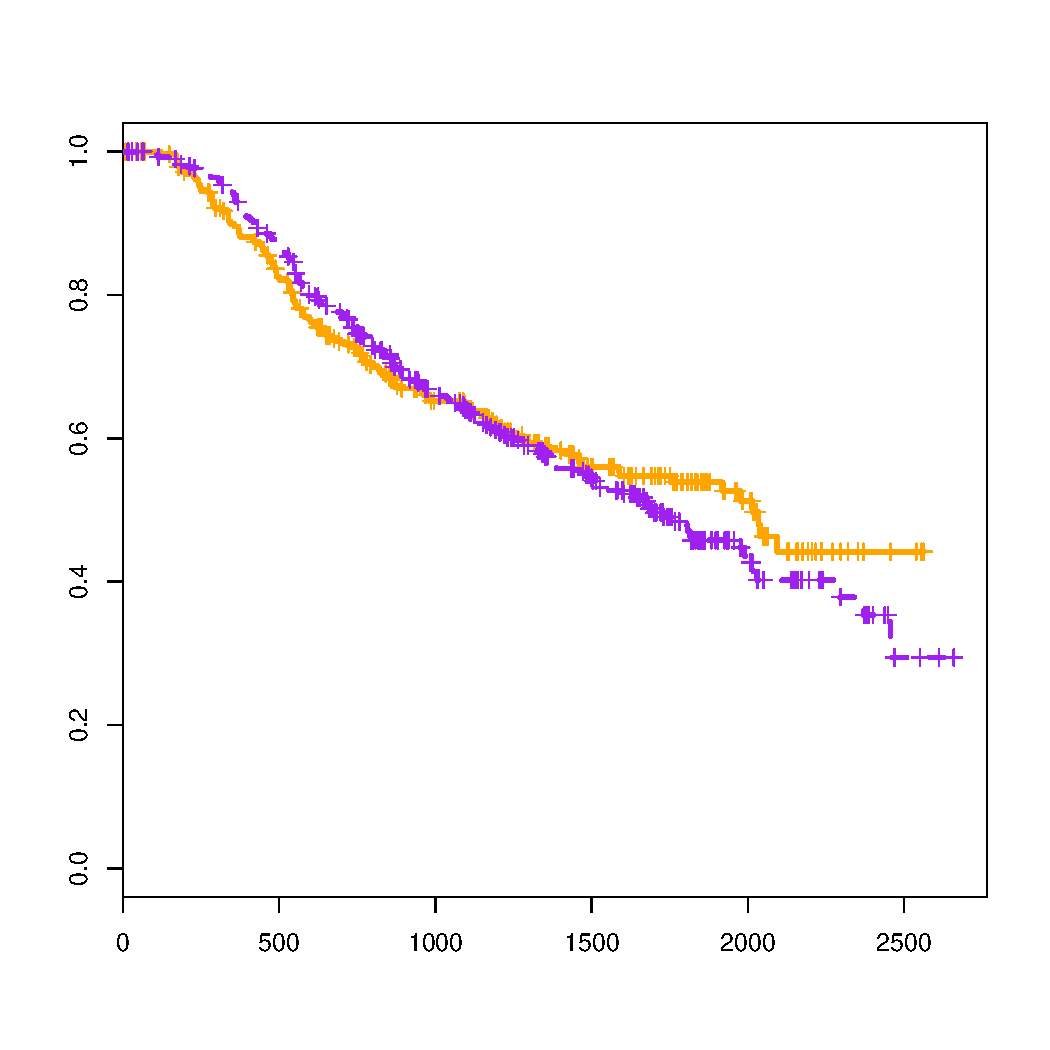
\includegraphics[width=0.18\textwidth, height=1.15in]{sc_meno.pdf}}
   \subfigure[\textsf{horm}]{
     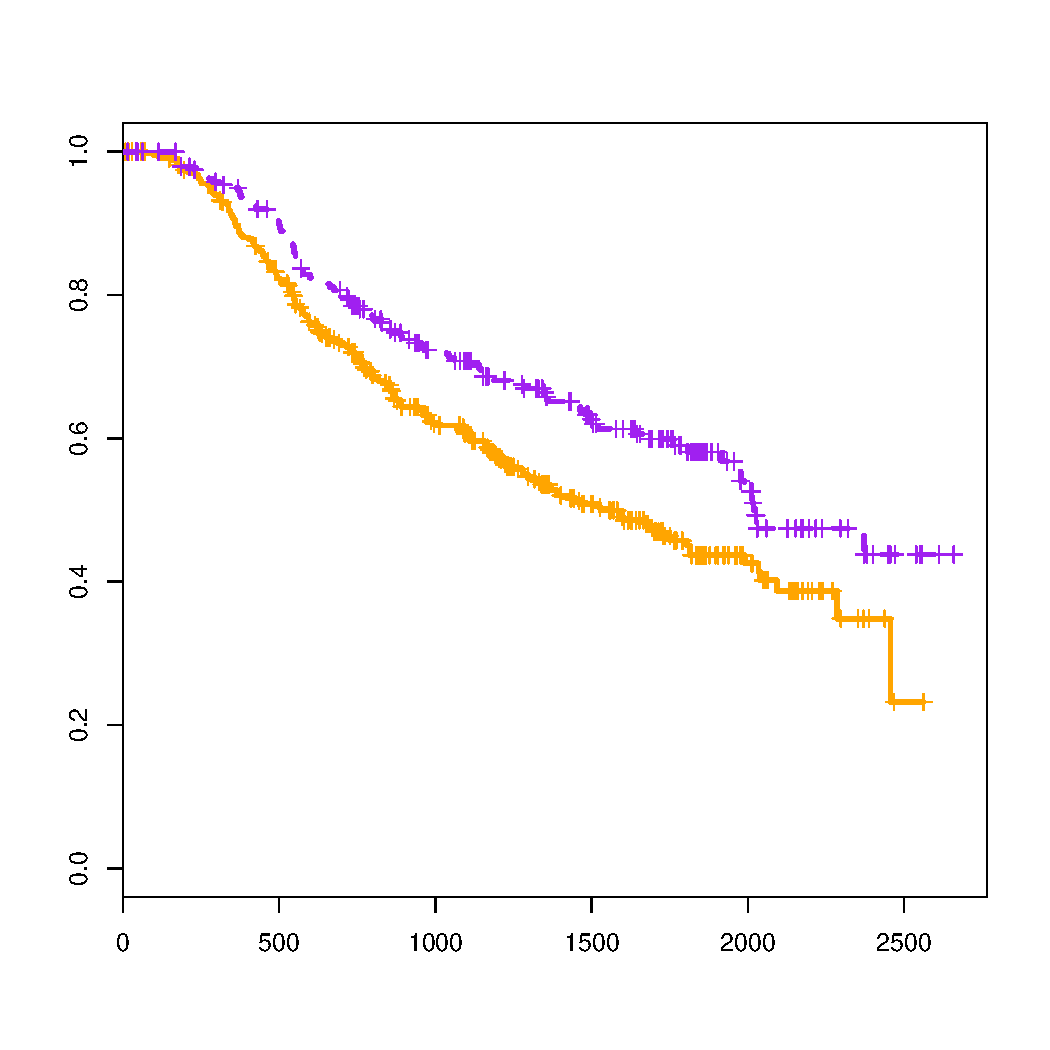
\includegraphics[width=0.18\textwidth, height=1.15in]{sc_horm.pdf}}
   \subfigure[\textsf{prog}]{
     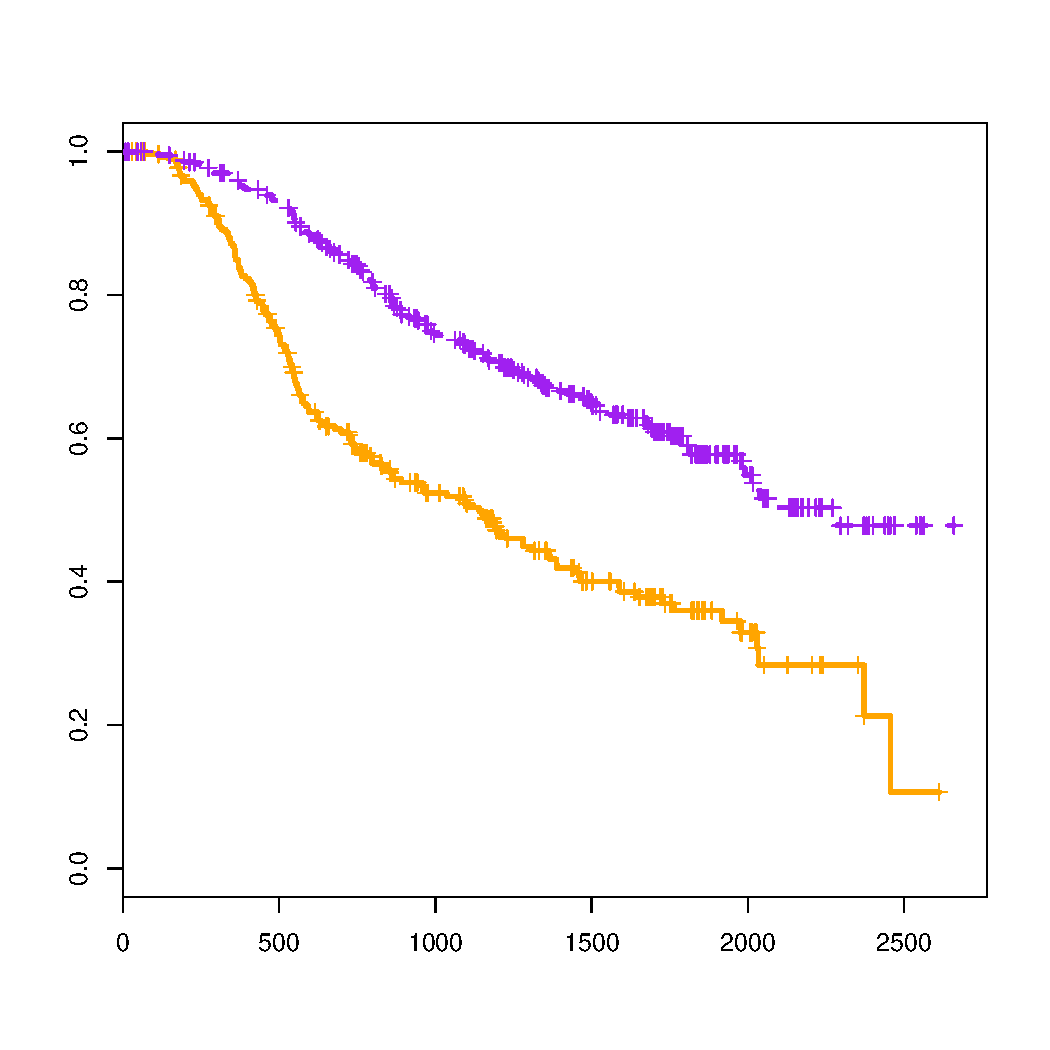
\includegraphics[width=0.18\textwidth, height=1.15in]{sc_prog.pdf}}
   \subfigure[\textsf{estr}]{
     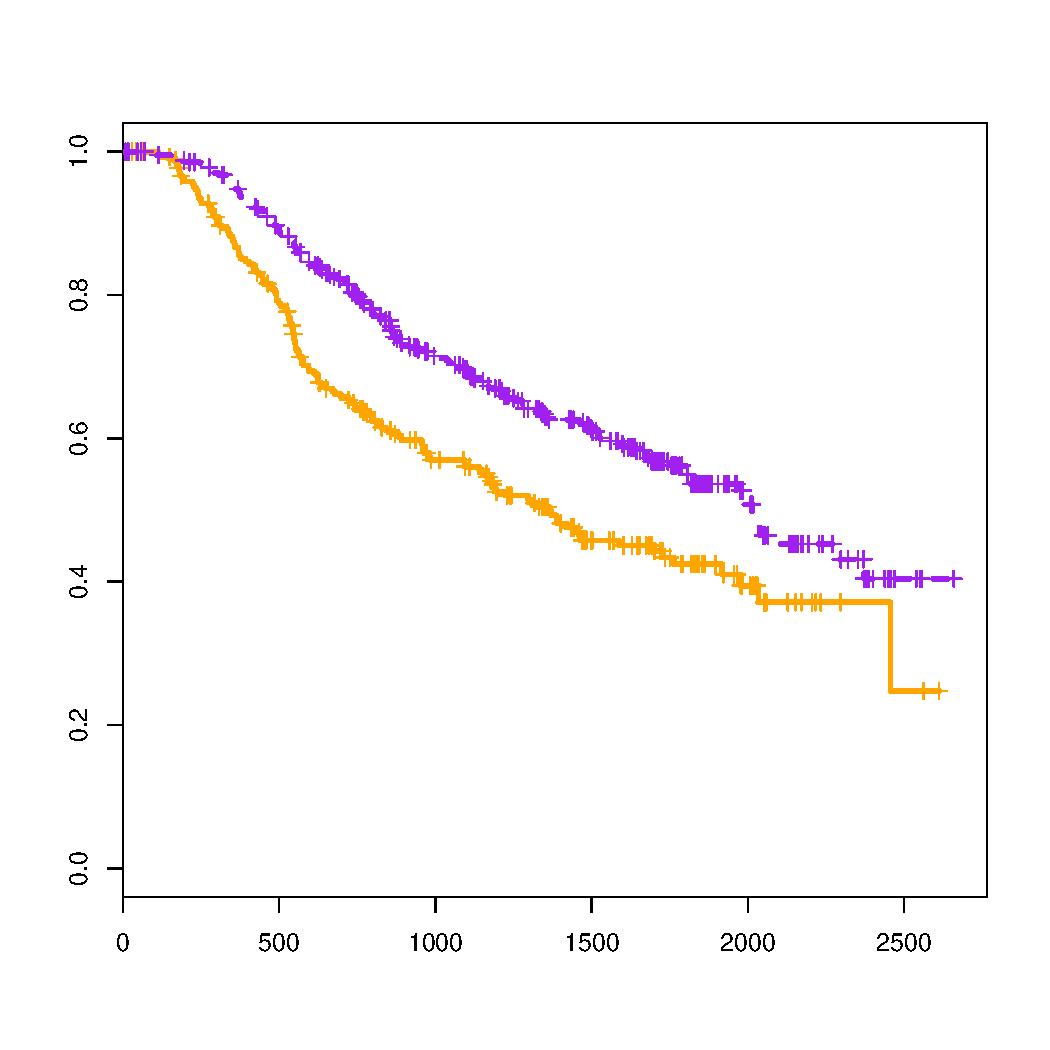
\includegraphics[width=0.18\textwidth, height=1.15in]{sc_estr.pdf}}
   \subfigure[\textsf{grade}]{
     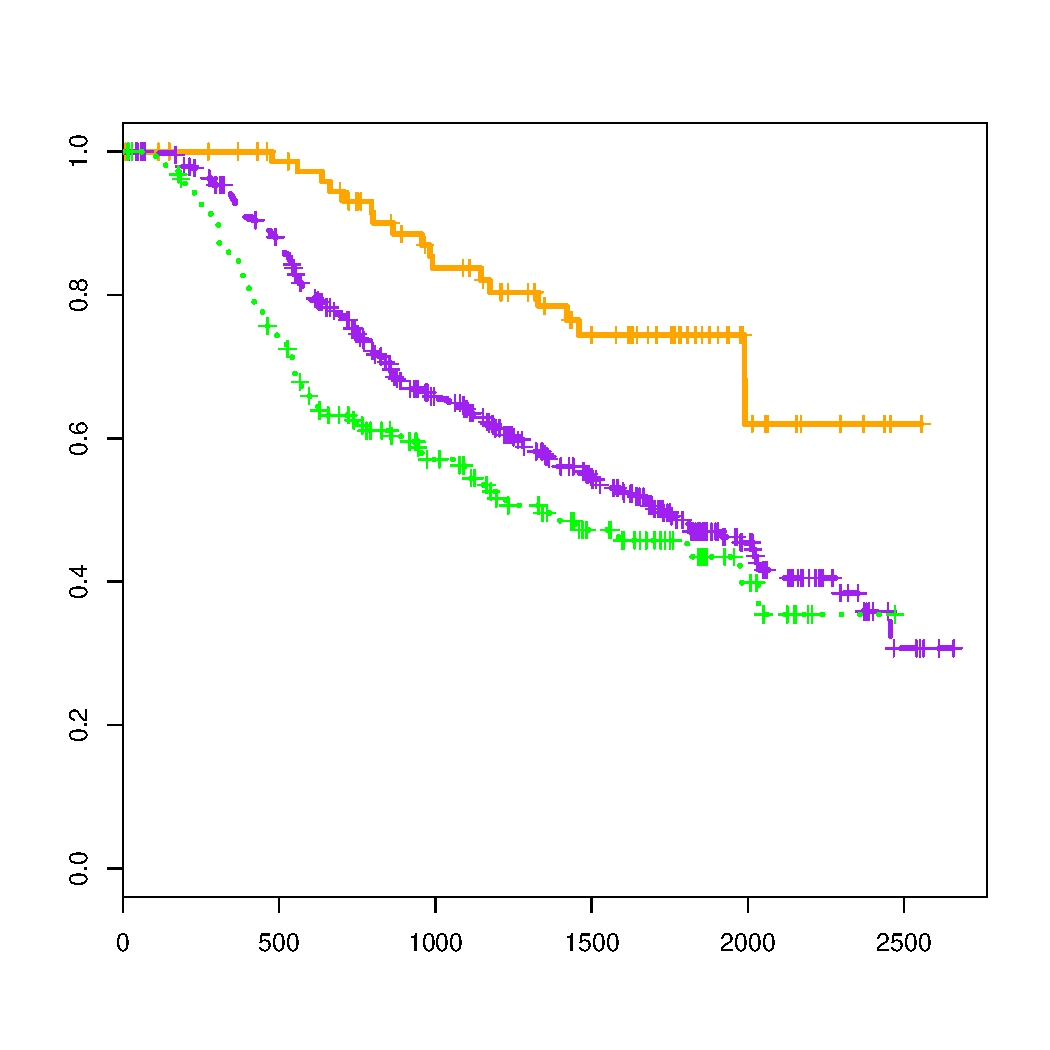
\includegraphics[width=0.18\textwidth, height=1.15in]{sc_grade.pdf}}
  \end{center}
  \vspace{-20pt}
  \label{fig:sc}
  \caption{Krzywe przeżycia Kaplana-Meiera dla zmiennych dyskretnych.}

\end{figure}

\begin{figure}[hbt!]
  \vspace{-10pt}
  \begin{center}
   \subfigure[\textsf{meno}]{
     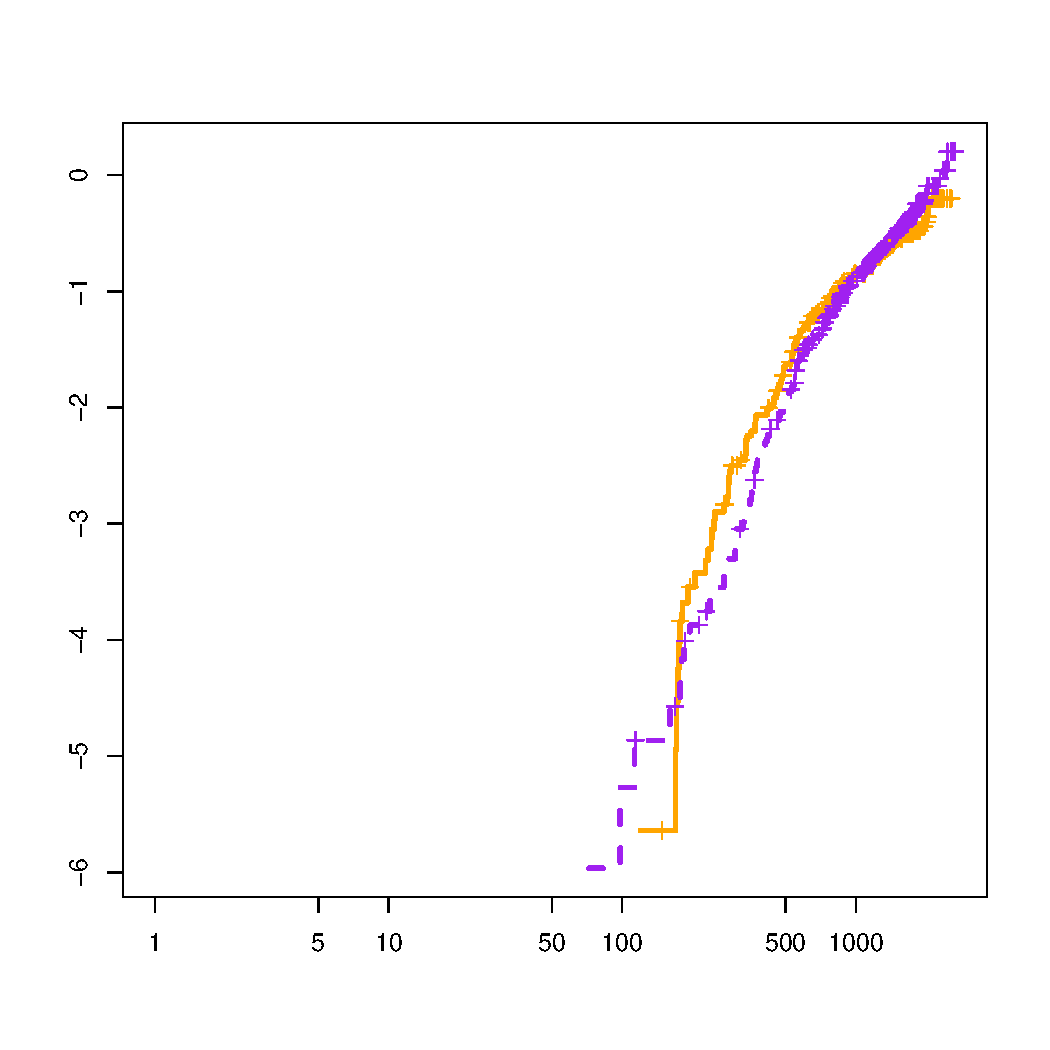
\includegraphics[width=0.18\textwidth, height=1.15in]{sc_meno_log.pdf}}
   \subfigure[\textsf{horm}]{
     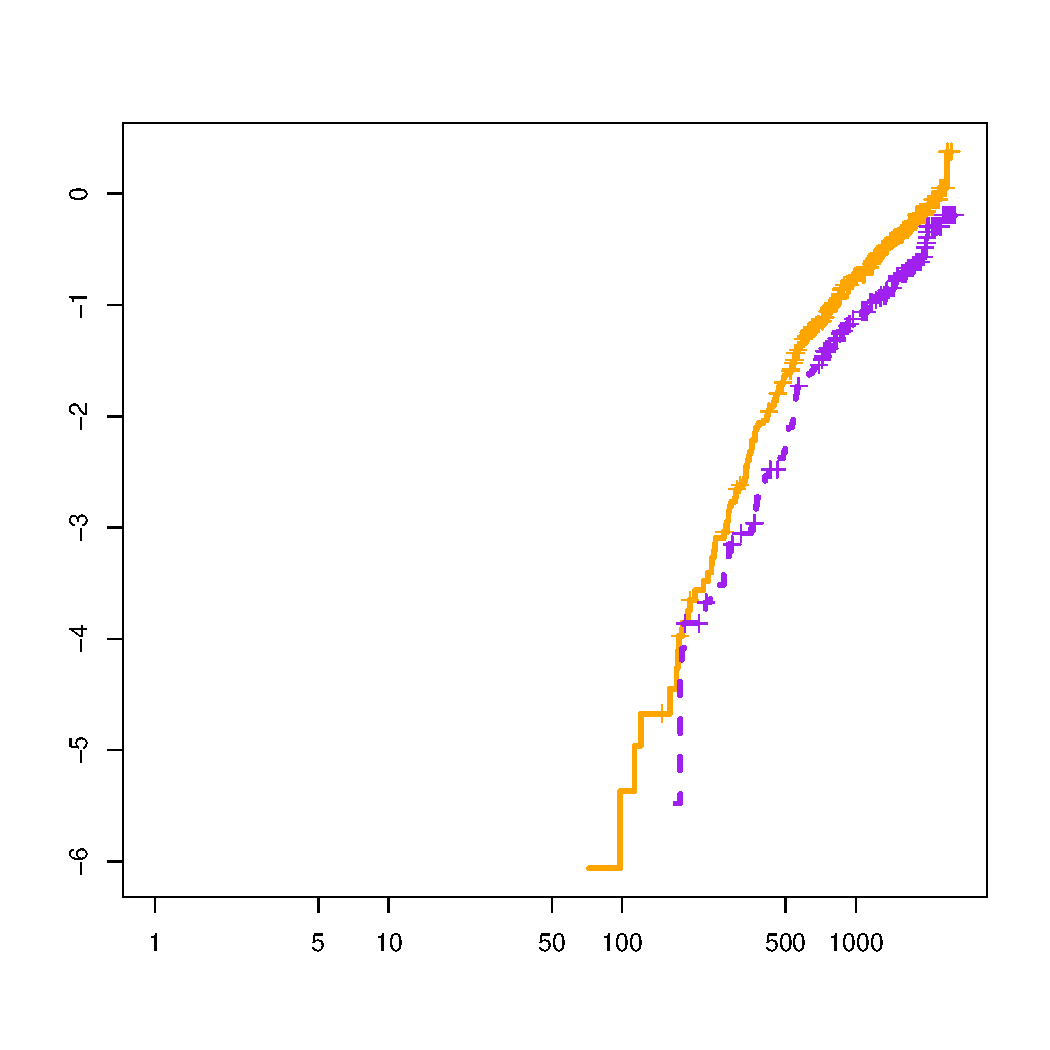
\includegraphics[width=0.18\textwidth, height=1.15in]{sc_horm_log.pdf}}
   \subfigure[\textsf{prog}]{
     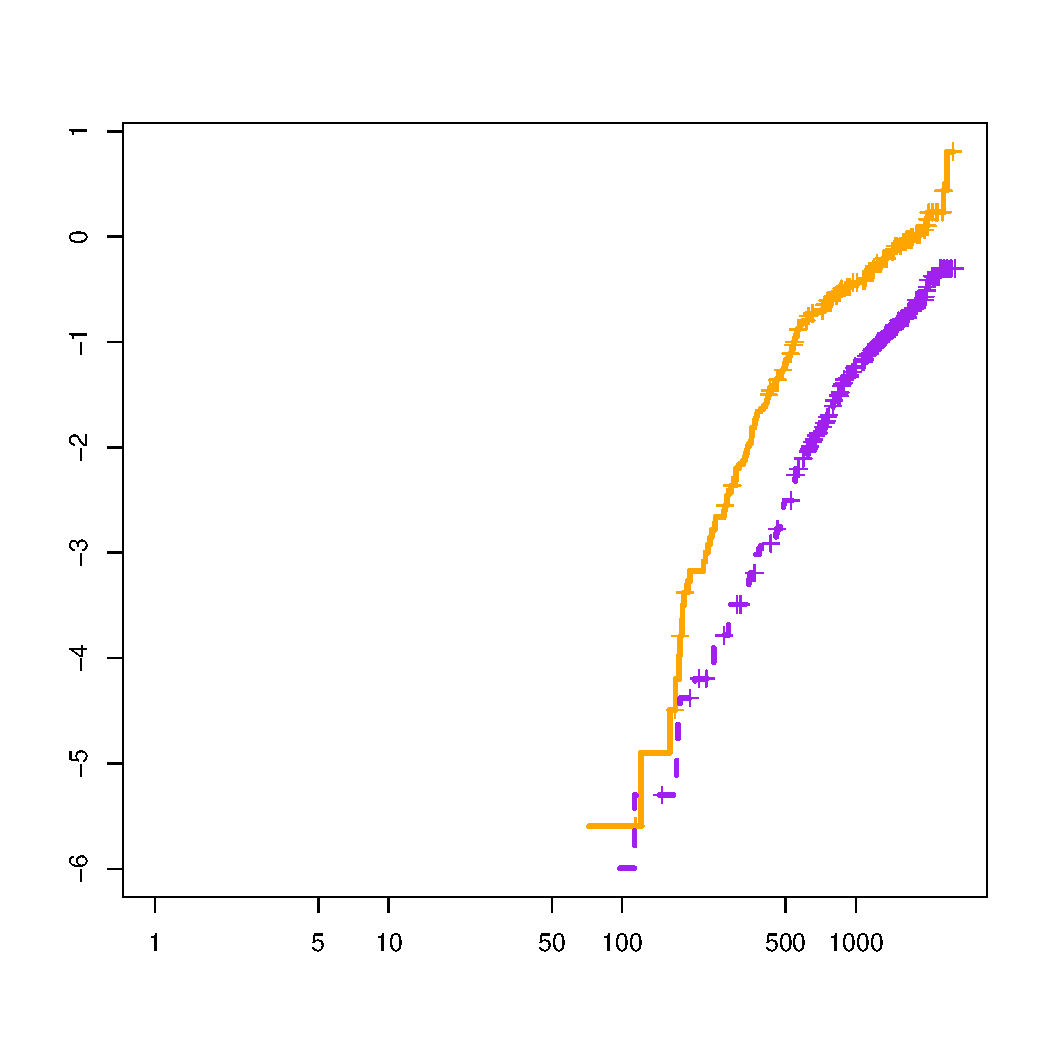
\includegraphics[width=0.18\textwidth, height=1.15in]{sc_prog_log.pdf}}
   \subfigure[\textsf{estr}]{
     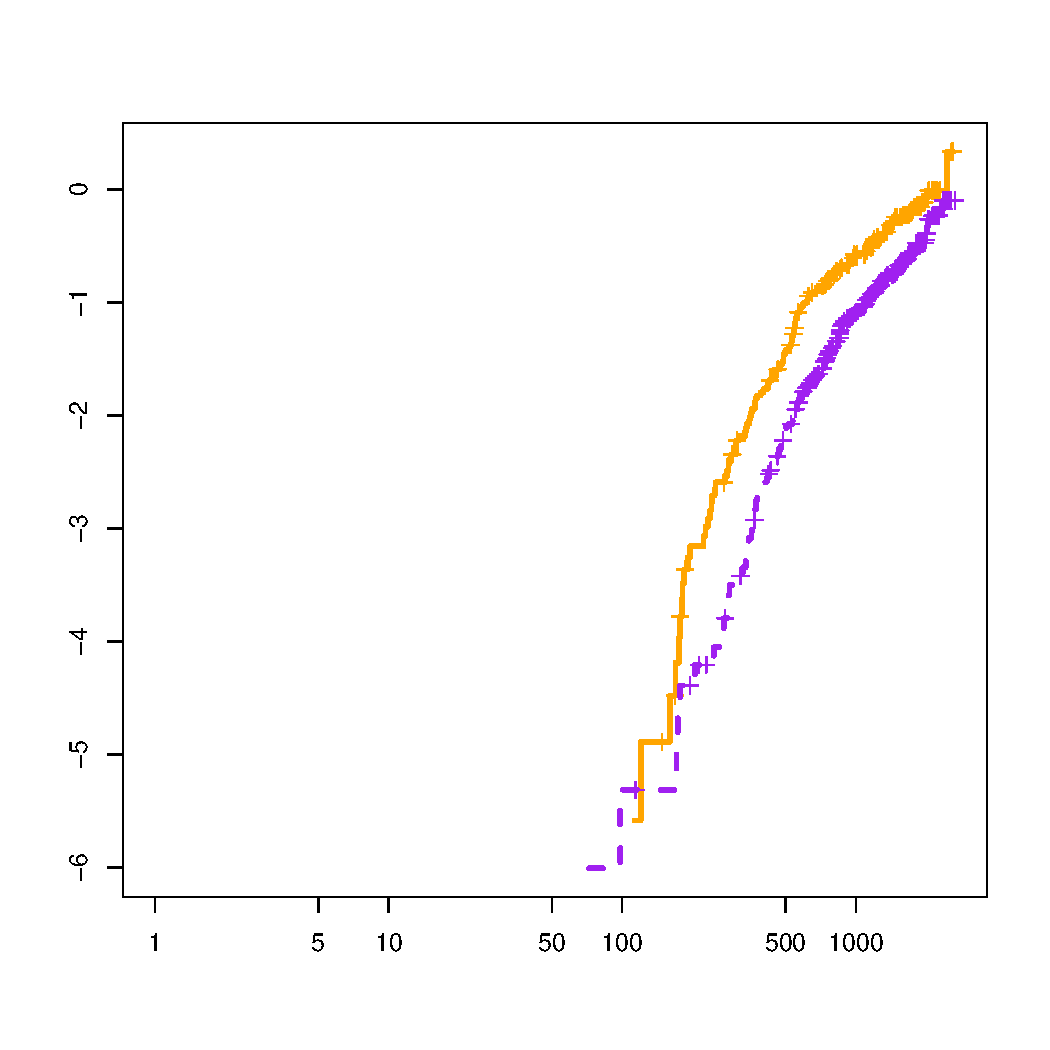
\includegraphics[width=0.18\textwidth, height=1.15in]{sc_estr_log.pdf}}
   \subfigure[\textsf{grade}]{
     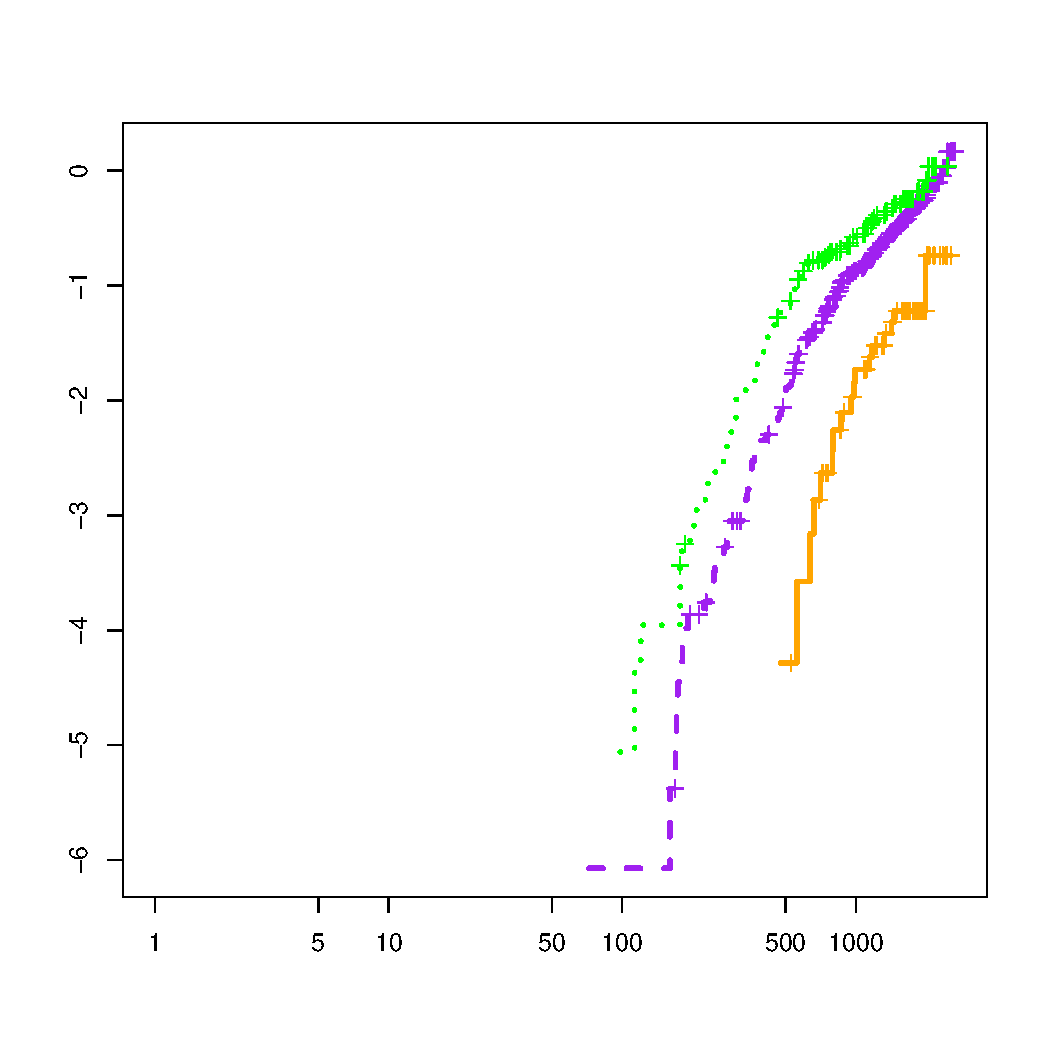
\includegraphics[width=0.18\textwidth, height=1.15in]{sc_grade_log.pdf}}
  \end{center}
  \vspace{-20pt}
  \label{fig:sc}
  \caption{Transformacje \textsf{log(-log)} krzywych przeżycia Kaplana-Meiera.}

\end{figure}

Krzywe przeżycia dla rożnych poziomów zmiennej \texttt{meno} przecinają
się, co może oznaczać niespełnianie założeń modelu PH. Dla pozostałych
zmiennych krzywe nie przecinają się oraz wykresy transformacji możemy
uznać za nieodstające od równoległych. Z tej racji proponujemy model
proporcjonalnych hazardów warstwowany względem zmiennej \texttt{meno},
gdyż nie ma podstaw by nie twierdzić, że założenia modelu ph nie są
spełnione.

\begin{wraptable}{r}{6.8cm}
\vspace{-20pt}
\caption{ Wyniki testów logrank. }
\begin{tabular}{lrrrrrr}
\toprule%
\ &$\chi^2$&St. swobody&p-wartość\\ \toprule meno&0.3&1&0.597\\ horm&8.6&1&0.003\\ prog&49.3&1&0.000\\ estr&14.3&1&0.000\\ grade&&2&\\  \bottomrule
\end{tabular}
\vspace{-7.5pt}
\end{wraptable}

W celu potwierdzenia wniosków płynących z graficznej prezentacji krzywych
przeżycia, przeprowadzono formalny test logrank dla każdej zmiennej,
którego podsumowanie widać w Tabeli 1. Dla zmiennej grade przeprowadzono
test logrank dla trendu z racji na naturalne uporządkowanie poziomów. Hipoteza zerowa zakłada, że krzywe przeżycia dla zmiennych nie różnią się istotnie statystycznie.
Wartości krytyczne dla zmiennych \textsf{horm}, \textsf{prog},
\textsf{estr} i \textsf{grade} \textbf{ (?-nie widzę p-wartości dla tej zmiennej :( }), które są mniejsze od zakładanego
poziomu istotności \(\alpha=0.05\) dają statystycznie istotne podstawy
do odrzucenia hipotez zerowych w testach logrank oraz do przyjęcia
hipotez alternatywnych o tym, że krzywe przeżycia dla tych zmiennych
różnią się. Dla zmiennej \textsf{meno} p-wartość \(0.597\) nie daje
podstaw do odrzucenia hipotezy zerowej (dla przyjętego poziomu istnotności \(\alpha=0.05\), mówiącej o równości krzywych przeżycia dla różnych poziomów tej
zmiennej.

\newpage
\textbf{Przekształcenia zmiennych ciągłych.} \newline
W celu sprawdzenia, czy zmienne ciągłe nie powinny zostać przekształcone
przed wprowadzeniem ich do modelu, wykonujemy wykresy reszt
martyngałowych pustego modelu od każdej z tych zmiennych. Wykresy
umieszczone na Rysunku 3 sugerują przekształcenie zmiennych poprzez
logarytm, więc dla potwierdzenia tych przypuszczeń narysowano dodatkowo 
wykresy reszt od logarytmów zmiennych i zaobserwowano, że wykresy są teraz
bliższe liniowym. Wprowadzono więc do modelu zmienne ciągłe
przekształcone logarytmem.

\begin{figure}[hbt!]
  \vspace{-10pt}
  \begin{center}
   \subfigure[\textsf{nodes}]{
     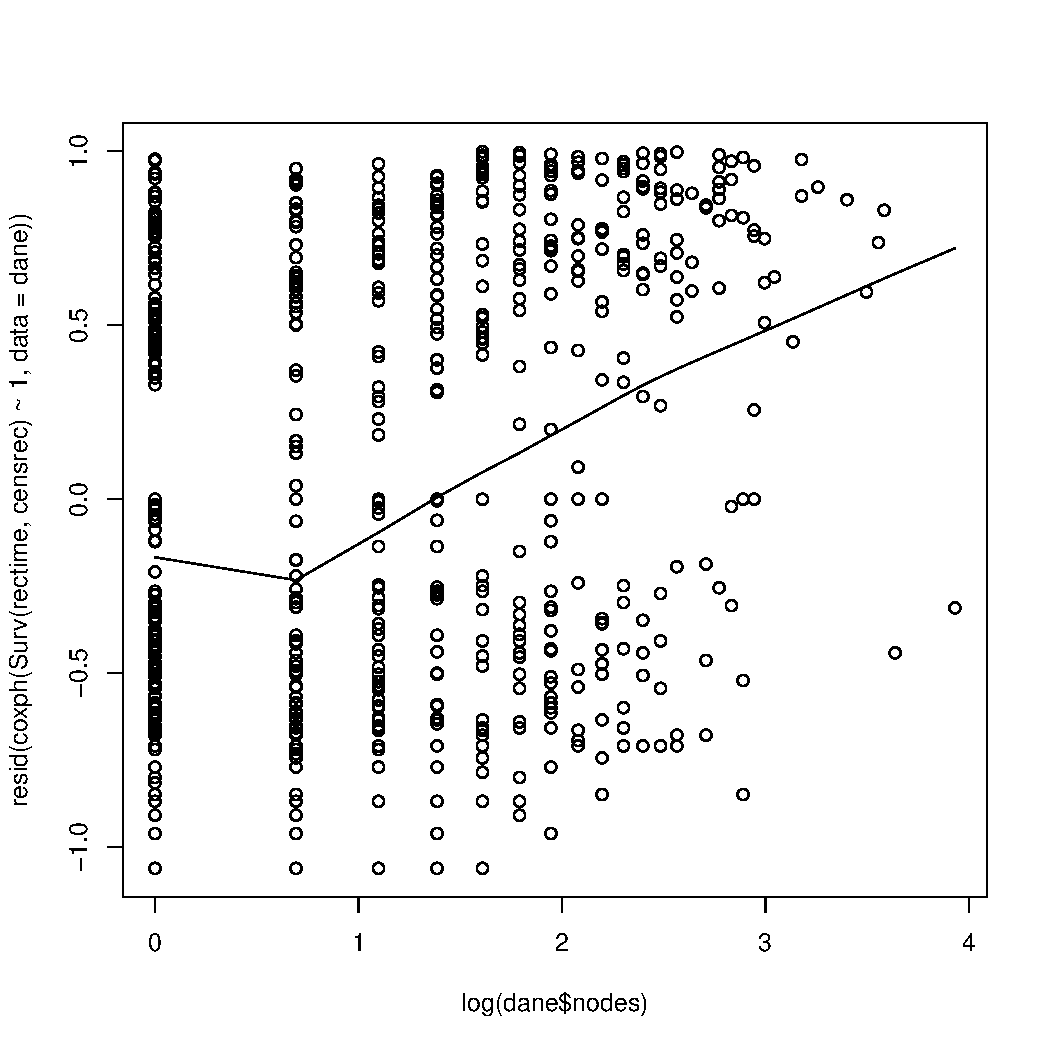
\includegraphics[width=0.32\textwidth, height=1.3in]{log_nodes.pdf}}
   \subfigure[\textsf{size}]{
     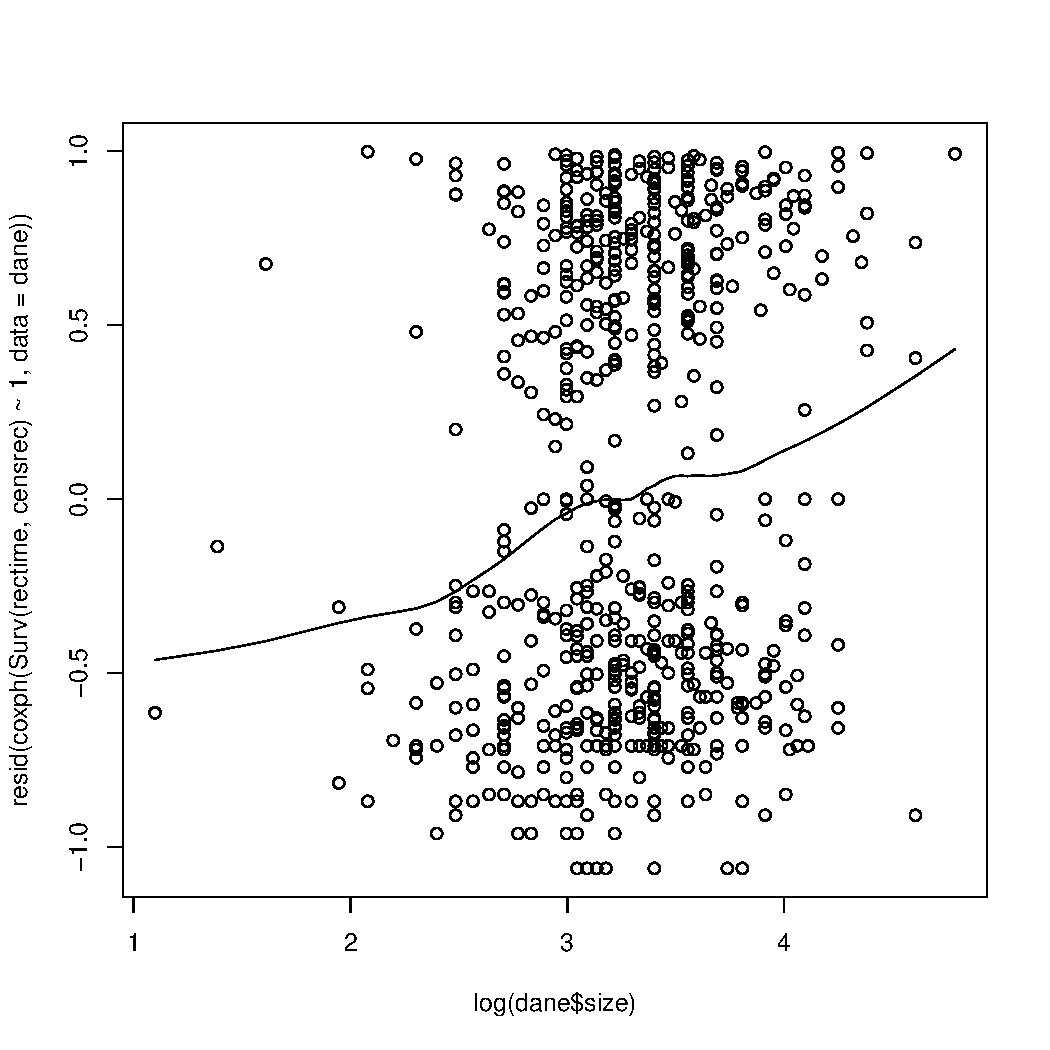
\includegraphics[width=0.32\textwidth, height=1.3in]{log_size.pdf}}
  \end{center}
  \vspace{-20pt}
  \label{fig:sc}
  \caption{Wykresy reszt martyngałowych od logarytmów zmiennych ciągłych.}

\end{figure}

\begin{wraptable}{r}{6.5cm}
\vspace{-12pt}
\caption{ Wyniki testu Schoenfelda. }
\begin{tabular}{lrrr}
\toprule%
  & $\rho$ & $\chi^2$ & p-wartość\\ \toprule 

horm & -0.008 & 0.019 & 0.891\\

prog & 0.036 & 0.376 & 0.540\\

estr & 0.071 & 1.483 & 0.223\\

grade & -0.083 & 1.826 & 0.177\\

log(size) & 0.008 & 0.020 & 0.888\\

log(nodes) & -0.049 & 0.799 & 0.372\\

GLOBAL & NA & 9.599 & 0.143\\  \bottomrule
\end{tabular}
\vspace{-7.5pt}
\end{wraptable}

\textbf{Sprawdzenie założeń - formalny test Schoenfelda.} \newline
W celu formalnego sprawdzenia czy współczynniki w modelu są stałe w
czasie przeprowadzono test Schoenfelda, którego globlna p-wartość oraz
pojedyncze p-wartości dla zmiennych dyskretnych oraz ciągłych
przekształconych przez logarytm są większe od zakładanego poziomu
istotności \(\alpha=0.05\) co nie daje podstaw do odrzucenia hipotezy
zerowej w tym teście, mówiącej o stałości współczynników w czasie.

Uwagę zwrócono również wykresom skalowanych reszt Schoenfelda dla
każdej zmiennej w modelu od czasu i dopasowano do nich krzywe. Dołączone granice dla 95\% obszarów ufności sugerują, że nie ma podstaw do odrzucenia hipotez, że krzywe nie różnią się od horyzontalnych.

\begin{figure}[hbt!]
\vspace{-10pt}
  \begin{center}
      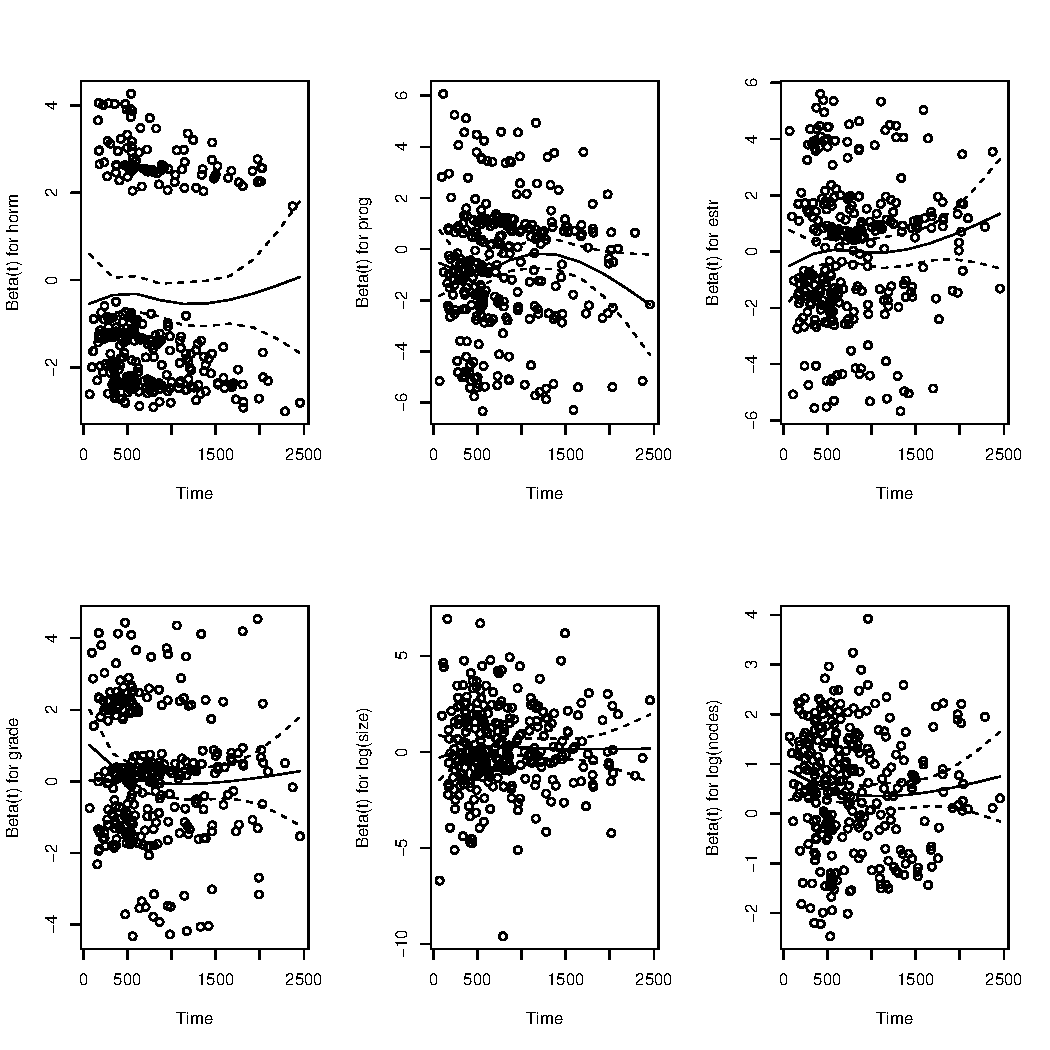
\includegraphics[width=0.85\textwidth, height=3in]{skal_res_shen.pdf}
      \caption{Wykresy skalowanych reszt Schoenfelda.}
   \end{center}
\end{figure}

Zarówno wykresy skalowanych reszt Schoenfelda, jak i wyniki testu nie
sugerują odstępstw od założenia PH.

\textbf{Dopasowanie modelu proporcjonalnych hazardów.} \newline

\begin{Shaded}
\begin{Highlighting}[]
\NormalTok{model <-}\StringTok{ }\KeywordTok{coxph}\NormalTok{(}\KeywordTok{Surv}\NormalTok{(rectime,censrec)~horm+prog+estr+grade+}\KeywordTok{strata}\NormalTok{(meno)+}\KeywordTok{log}\NormalTok{(size)+}\KeywordTok{log}\NormalTok{(nodes), }
               \DataTypeTok{data =} \NormalTok{dane) }
\KeywordTok{summary}\NormalTok{(model)}
\end{Highlighting}
\end{Shaded}

\begin{verbatim}
Call:
coxph(formula = Surv(rectime, censrec) ~ horm + prog + estr + 
    grade + strata(meno) + log(size) + log(nodes), data = dane)

  n= 686, number of events= 299 

               coef exp(coef) se(coef)      z Pr(>|z|)    
horm       -0.39218   0.67558  0.12913 -3.037  0.00239 ** 
prog       -0.69283   0.50016  0.14570 -4.755 1.98e-06 ***
estr        0.03958   1.04038  0.14379  0.275  0.78309    
grade       0.15096   1.16295  0.11237  1.343  0.17914    
log(size)   0.19191   1.21156  0.13175  1.457  0.14523    
log(nodes)  0.48933   1.63123  0.06690  7.314 2.59e-13 ***
---
Signif. codes:  0 '***' 0.001 '**' 0.01 '*' 0.05 '.' 0.1 ' ' 1

           exp(coef) exp(-coef) lower .95 upper .95
horm          0.6756     1.4802    0.5245    0.8702
prog          0.5002     1.9994    0.3759    0.6655
estr          1.0404     0.9612    0.7849    1.3791
grade         1.1630     0.8599    0.9331    1.4495
log(size)     1.2116     0.8254    0.9358    1.5685
log(nodes)    1.6312     0.6130    1.4308    1.8598

Concordance= 0.696  (se = 0.025 )
Rsquare= 0.169   (max possible= 0.99 )
Likelihood ratio test= 126.9  on 6 df,   p=0
Wald test            = 128.6  on 6 df,   p=0
Score (logrank) test = 135.3  on 6 df,   p=0
\end{verbatim}

W stworzonym modelu zmiennymi istotnymi statystycznie na poziomie
istotności \(0.05\) są: \texttt{horm}, \texttt{prog},
log(\texttt{nodes}). Współczynniki modelu przy tych zmiennych wynoszą
odpowiednio: \(-0.39, -0.69, 0.49\). Oznacza to, że jeśli została użyta
terapia hormonalna, to hazard zgonu lub nawrotu choroby zmniejsza się
\(\exp(-0.39)=0.68\) raza w stosunku nieużycia terapii hormonalnej
(gdy wszystkie inne zmienne są takie same). Jeśli wskaźnik receptorów
progesteronu zmienia się z ujemnego na dodatni, to hazard zmieni się o
\(\exp(-0.69)=0.5\) raza, natomiast gdy logarytm liczby węzłów chłonnych
z przerzutami nowotworu wzrośnie o 1, to hazard zwiększy się
\(\exp(0.49)=1.63\) raza, gdy wszystkie inne zmienne pozostaną na tym samym poziomie.

Testy Likelihood, Wald i Score dają p-wartość mniejszą od 0.05 (przyjętego poziomu istotności), co wskazuje, że odrzucamy hipotezę zerową na rzecz hipotezy alternatywnej, zatem dopasowany model jest istotnie lepszy od modelu pustego. 

\newpage
\textbf{Sprawdzenie dopasowania modelu proporcjonalnych hazardów.}
\newline
W celu sprawdzenia dopasowania modelu narysowano wykresy reszt
dewiancji i martyngałowych od liniowej kombinacji zmiennych oraz indeksów. Na
żadnym z wykresów nie można wskazać wyraźnie odstających reszt
(\textcolor{red}{a wykres d?}). Wykres reszt dewiancji od indeksów można
uznać za symetryczny, pozostałe niekoniecznie, co sugeruje, że
dopasowany model nie jest perfekcyjny.

\begin{figure}[hbt!]
  \vspace{-10pt}
  \begin{center}
   \subfigure[Reszty dewiancji a indeks.]{
     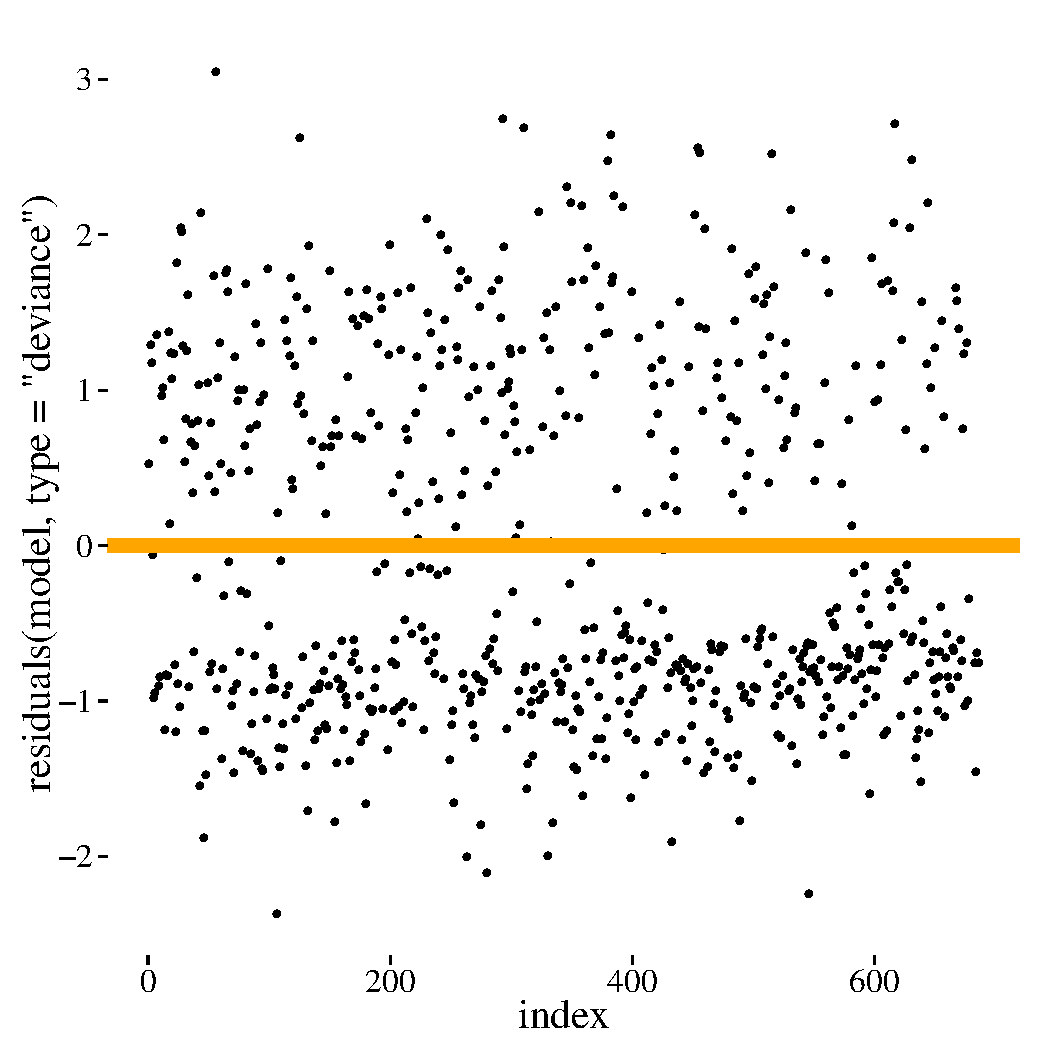
\includegraphics[width=0.48\textwidth, height=2in]{res_ind_dev.pdf}}
   \subfigure[Reszty martyngałowe a indeks.]{
     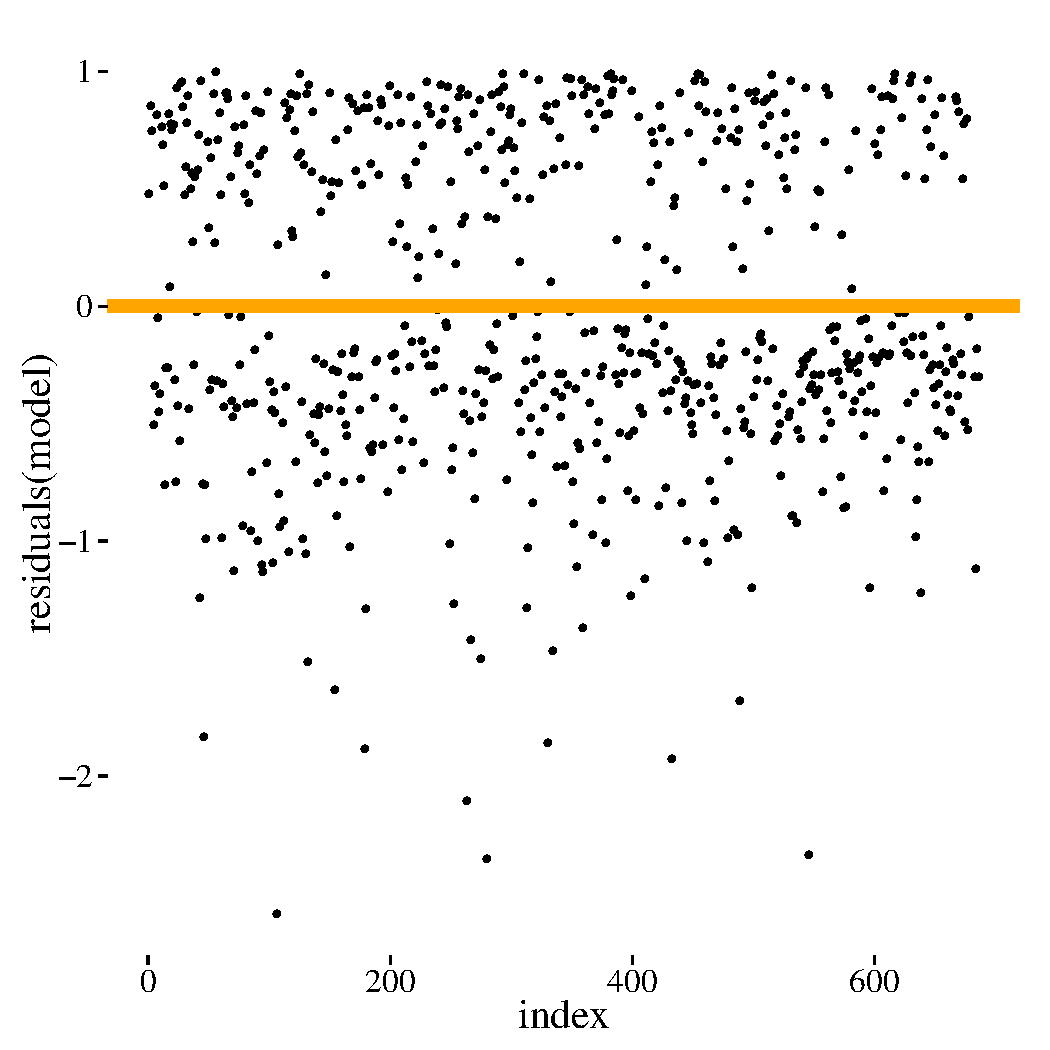
\includegraphics[width=0.48\textwidth, height=2in]{res_ind_mart.pdf}}
   \subfigure[Reszty dewiancji a liniowe kombinacje.]{
     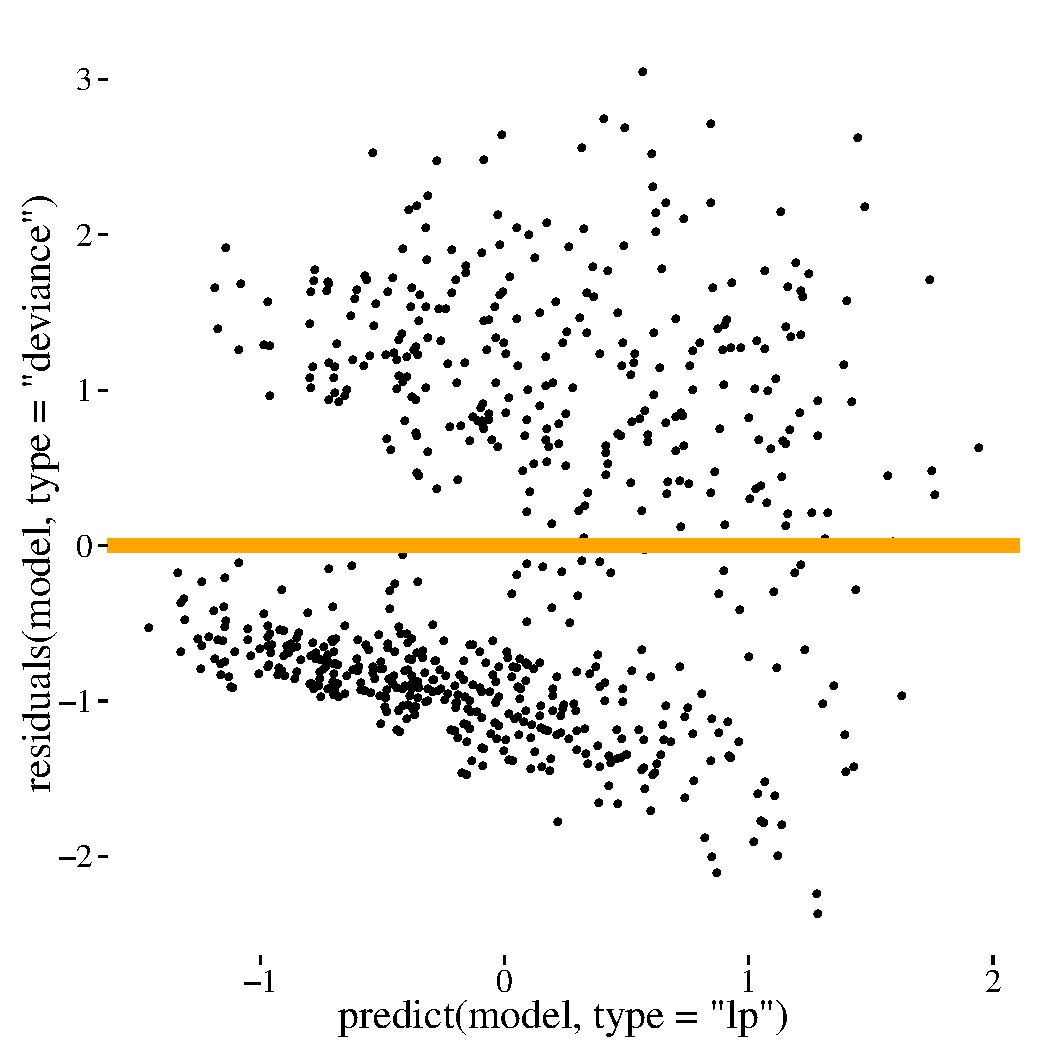
\includegraphics[width=0.48\textwidth, height=2in]{res_lp_dev.pdf}}
   \subfigure[Reszty martyngałowe a liniowe kombinacje.]{
     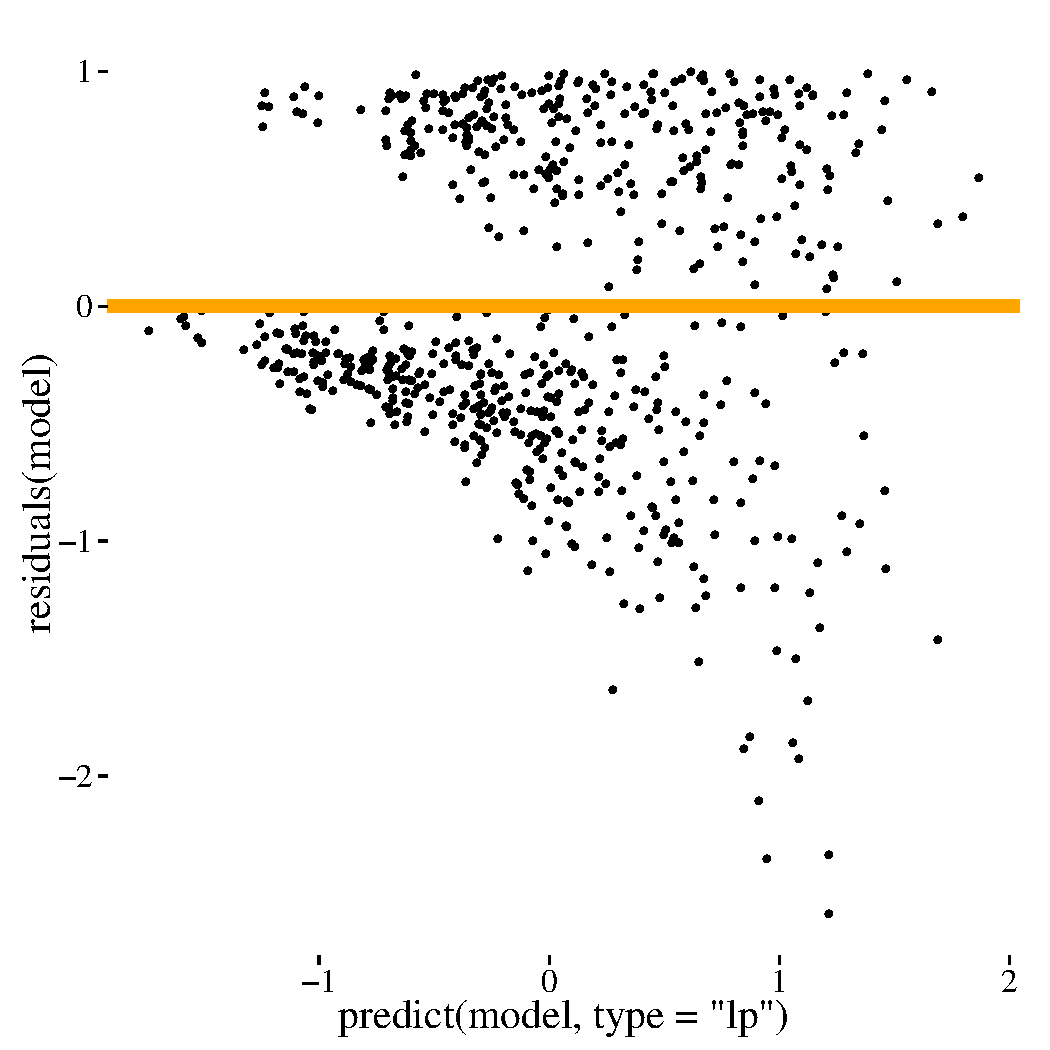
\includegraphics[width=0.48\textwidth, height=2in]{res_lp_mart.pdf}}
  \end{center}
  \vspace{-20pt}
  \label{fig:sc}
  \caption{Wykresy reszt martyngałowych i dewiancji.}

\end{figure}

\newpage
\textbf{Kody.} \newline

\begin{Shaded}
\begin{Highlighting}[]
\KeywordTok{library}\NormalTok{(foreign)}
\NormalTok{dane <-}\StringTok{ }\KeywordTok{read.dta}\NormalTok{(}\StringTok{"gbcs_short.dta"}\NormalTok{)}
\KeywordTok{library}\NormalTok{(survival)}
\KeywordTok{plot}\NormalTok{(}\KeywordTok{survfit}\NormalTok{(}\KeywordTok{Surv}\NormalTok{(rectime,censrec)~meno, }\DataTypeTok{data =} \NormalTok{dane), }\DataTypeTok{col=}\KeywordTok{c}\NormalTok{(}\StringTok{"orange"}\NormalTok{,}\StringTok{"purple"}\NormalTok{), }\DataTypeTok{lty=}\KeywordTok{c}\NormalTok{(}\DecValTok{1}\NormalTok{:}\DecValTok{2}\NormalTok{), }\DataTypeTok{lwd=}\DecValTok{3}\NormalTok{)}
\CommentTok{#...}
\KeywordTok{plot}\NormalTok{(}\KeywordTok{log}\NormalTok{(dane$size), }\KeywordTok{resid}\NormalTok{(}\KeywordTok{coxph}\NormalTok{(}\KeywordTok{Surv}\NormalTok{(rectime,censrec)~}\DecValTok{1}\NormalTok{, }\DataTypeTok{data =} \NormalTok{dane)))}
\KeywordTok{lines}\NormalTok{(}\KeywordTok{lowess}\NormalTok{(}\KeywordTok{log}\NormalTok{(dane$size), }\KeywordTok{resid}\NormalTok{(}\KeywordTok{coxph}\NormalTok{(}\KeywordTok{Surv}\NormalTok{(rectime,censrec)~}\DecValTok{1}\NormalTok{, }\DataTypeTok{data =} \NormalTok{dane)), }\DataTypeTok{iter =} \DecValTok{0}\NormalTok{, }\DataTypeTok{f =} \FloatTok{0.6}\NormalTok{))}
\CommentTok{#...}

\KeywordTok{par}\NormalTok{(}\DataTypeTok{mfrow=}\KeywordTok{c}\NormalTok{(}\DecValTok{2}\NormalTok{,}\DecValTok{3}\NormalTok{))}
\KeywordTok{plot}\NormalTok{(}\KeywordTok{cox.zph}\NormalTok{(model, }\DataTypeTok{transform =} \StringTok{"identity"}\NormalTok{), }\DataTypeTok{df=}\DecValTok{4}\NormalTok{,}\DataTypeTok{nsmo=}\DecValTok{10}\NormalTok{, }\DataTypeTok{se=}\OtherTok{TRUE}\NormalTok{)}
\NormalTok{model <-}\StringTok{ }\KeywordTok{coxph}\NormalTok{(}\KeywordTok{Surv}\NormalTok{(rectime,censrec)~horm+prog+estr+grade+}\KeywordTok{strata}\NormalTok{(meno)+}\KeywordTok{log}\NormalTok{(size)+}\KeywordTok{log}\NormalTok{(nodes), }
               \DataTypeTok{data =} \NormalTok{dane) }
\KeywordTok{summary}\NormalTok{(model)}

\CommentTok{#...}
\KeywordTok{qplot}\NormalTok{(}\DecValTok{1}\NormalTok{:}\DecValTok{686}\NormalTok{,}\KeywordTok{residuals}\NormalTok{(model, }\DataTypeTok{type=}\StringTok{"deviance"}\NormalTok{))+}\KeywordTok{xlab}\NormalTok{(}\StringTok{"index"}\NormalTok{)+}\KeywordTok{theme_tufte}\NormalTok{(}\DataTypeTok{base_size=}\DecValTok{20}\NormalTok{)+}\KeywordTok{geom_hline}\NormalTok{()+}
\StringTok{   }\KeywordTok{geom_hline}\NormalTok{(}\DataTypeTok{yintercept=}\DecValTok{0}\NormalTok{, }\DataTypeTok{col =}\StringTok{"orange"}\NormalTok{, }\DataTypeTok{size =} \DecValTok{3}\NormalTok{)}
\end{Highlighting}
\end{Shaded}

\end{document}
